% \documentclass{article}

% % Language setting
% % Replace `english' with e.g. `spanish' to change the document language
% \usepackage[english, russian]{babel}

% % Set page size and margins
% % Replace `letterpaper' with `a4paper' for UK/EU standard size
% \usepackage[letterpaper,top=2cm,bottom=2cm,left=3cm,right=3cm,marginparwidth=1.75cm]{geometry}

% % Useful packages
% \usepackage{amsmath}
% \usepackage{color}
% \usepackage{xcolor}
% \usepackage[dvipsnames]{xcolor}
% \usepackage{graphicx}
% \usepackage[colorlinks=true, allcolors=blue]{hyperref}
% \usepackage{color}   %May be necessary if you want to color links
% \usepackage{hyperref}
% \hypersetup{
%     colorlinks=true, %set true if you want colored links
%     linktoc=all,     %set to all if you want both sections and subsections linked
%     linkcolor=blue,  %choose some color if you want links to stand out
% }
\documentclass{article}

% Language setting
% Replace `english' with e.g. `spanish' to change the document language
\usepackage[english,russian]{babel}
\usepackage{amsmath}

%графика
\usepackage{wrapfig}
\usepackage{graphicx}
\usepackage{pgfplots}
\usepackage{tikz}


\usepackage{tcolorbox}

% Set page size and margins
% Replace `letterpaper' with `a4paper' for UK/EU standard size
\usepackage[letterpaper,top=2cm,bottom=2cm,left=3cm,right=3cm,marginparwidth=1.75cm]{geometry}

% Useful packages
\usepackage{amsmath}
\usepackage{amssymb}
\usepackage{graphicx}
\usepackage{fixltx2e}
\usepackage[colorlinks=true, allcolors=blue]{hyperref}

\usepackage{geometry}
\geometry{left=25mm,right=25mm,
 top=25mm,bottom=25mm}

\title{Торговля опционами 2}
\author{Бидва Максим}
% Колонтитулы
\usepackage{fancyhdr}
\pagestyle{fancy}
\renewcommand{\headrulewidth}{0.1mm}  
\renewcommand{\footrulewidth}{0.1mm}
\lfoot{}
\rfoot{\thepage}
\cfoot{}
\rhead{CMF-2022}
\chead{}




\begin{document}
\maketitle
\tableofcontents
\newpage
\section{Кратко про прошлую лекцию}
\begin{multicols}
    \begin{itemize}
        \item Что такое опцион, Put/Call
        \item Говорили только про валютные ванильные опционы
        \item Мы с помощью бинарного дерева поняли Market Value опциона
        \item MV не уменьшается с увеличением волатильности
        \item Немножко поговорили про то как рынки устроены
    \end{itemize}
\end{multicols}

\section{Греки}

Греки(Greeks) официально это производные Market Value продуктов по разным по сути вещам(это могут быть производные любого порядка).\\
Greeks Delta = $\frac{\partial MV}{\partial S}$
\section{MV и Delta в момент экспирации}
У синего и красного опционов известны время до исполнения, номинал и страйк.\\
\textcolor{red}{USD Call, RUB Put, $T_e = 1w$, N = 10m\$, k = 73}\\
\textcolor{blue}{USD Put, RUB Call, $T_e = 1w$, N = 10m\$, k = 73}

\begin{center}
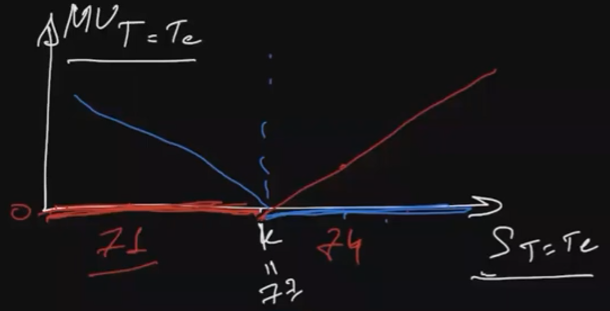
\includegraphics[width=300pt]{picture_1.png}\\
\caption{Зависимость цены опциона от спота в момент исполнения}\\
\bigskip
\bigskip
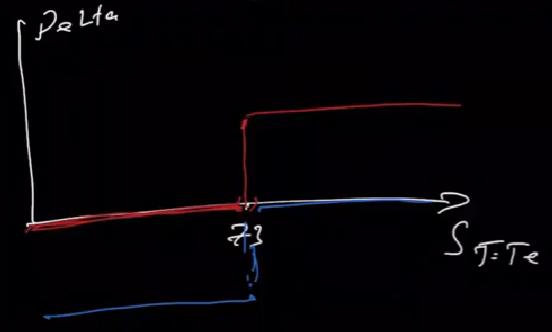
\includegraphics[width=300pt]{picture_2.png}\\
\caption{Зависимость дельты от спота в момент исполнения}\\

\end{center}    

\section{MV и Delta до экспирации}
Пусть теперь мы хотим понять что происходит не в момент исполнения опциона, а за какое-то время до.
Путь T < \textcolor{blue}{T} < \textcolor{red}{T} < \textcolor{orange}{T} - 4 времени до исполнения Call опциона со страйком k
\begin{center}
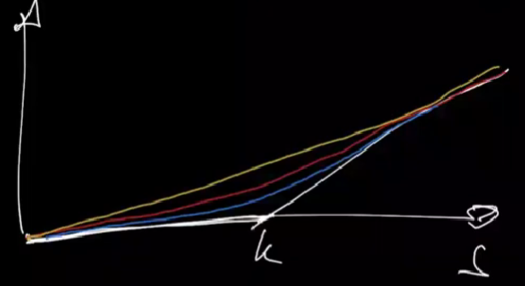
\includegraphics[width=300pt]{picture_3.png}\\
\caption{Зависимость цены опциона от спота за T, \textcolor{blue}{T}, \textcolor{red}{T}, \textcolor{orange}{T} до исполнения}\\
\bigskip
\bigskip
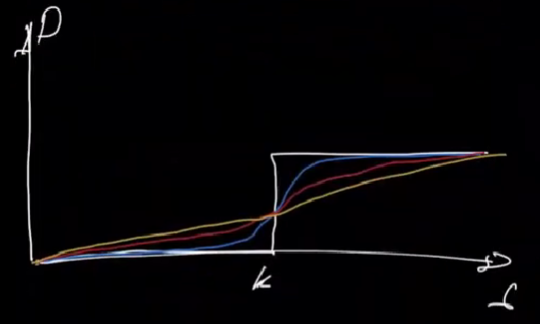
\includegraphics[width=300pt]{picture_4.png}\\
\caption{Зависимость дельты от спота за T, \textcolor{blue}{T}, \textcolor{red}{T}, \textcolor{orange}{T} до исполнения}\\

\end{center}  
\newpage
\section{Матовое стекло}
Нарисовали следующий график на бумаге:
\begin{center}  
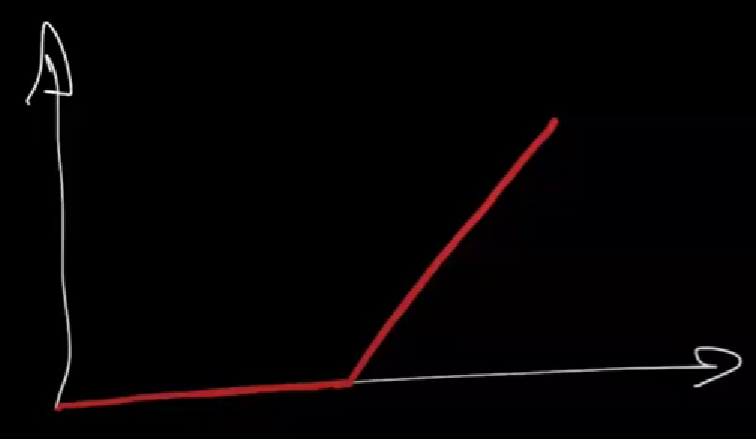
\includegraphics[width=300pt]{picture_5.png}\\
\end{center}  
Положим матовое стекло на бумагу, тогда бы будем идеально видеть график.\\
Теперь начнём отодвигать матовое стекло и смотреть через него на график. \\
Обведенные части не особо поменяются.\\
Углы размоются(как на картинке ниже).\\
\begin{center}  
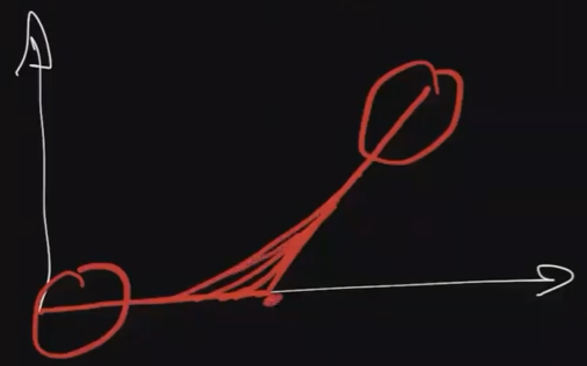
\includegraphics[width=300pt]{picture_6.png}\\
\end{center}  

Это ровно повторяет эволюцию кривых зависимости MV от спота при изменении времени до экспирации.\\
\newpage
Аналогичное верно и для зависимости Дельты от спота при изменении времени до экспирации.\\
\begin{center}  
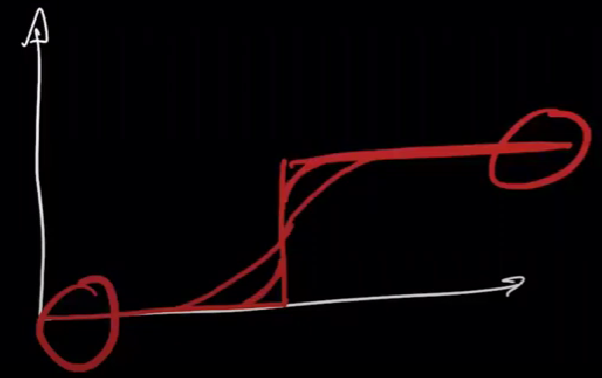
\includegraphics[width=300pt]{picture_7.png}\\
\end{center}  

Так же сглаживаются все греки.\\
Картинка для грека Vanna(подробнее про него дальше в конспекте):
%Аналогично и грек Vanna сглаживается с уменьшением времени до экспирации.
\begin{center}  
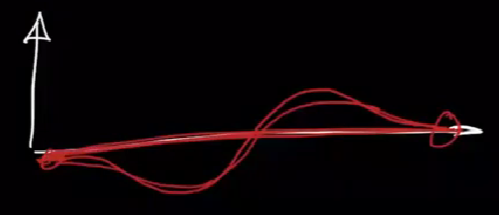
\includegraphics[width=300pt]{picture_9.png}\\
\end{center}  
Увеличение времени до экспирации $\sim$ увеличению волатильности.($T_1 > T_2 \sim G_1 > G_2$)\\
Матовое стекло устроено так: у него одна поверхность ровная, а другая рандомная. А луч света проходя через это стекло меняется следующим образом:
\begin{center}  
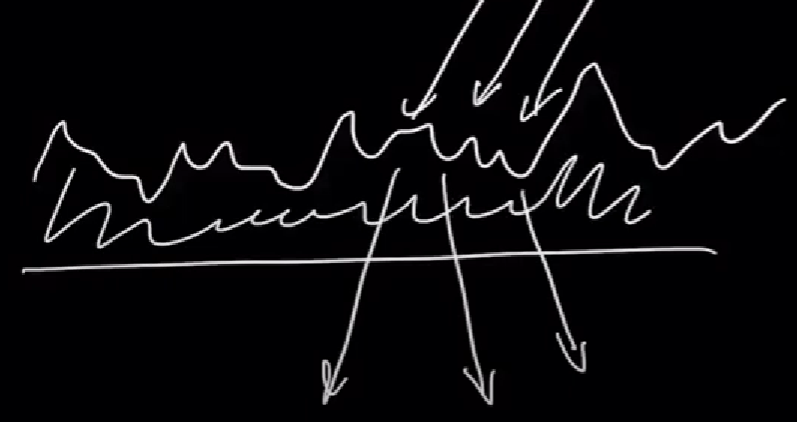
\includegraphics[width=300pt]{picture_8.png}\\
\end{center}  
\newpage
\section{Delta Bleed}
Пусть у нас есть опцион USD RUB Call, k=73, s = 72, T = 2d, N = 100m\$, $D_1$ - его дельта.\\
Мы держим против него Short с дельтой $D_1$, чтобы суммарно дельта была 0.\\
Мы приходим на следующее утро, видим, что у нас Дельта портфеля не 0, а отрицательная.\\(s = 72, T = 1d)\\
\begin{center}  
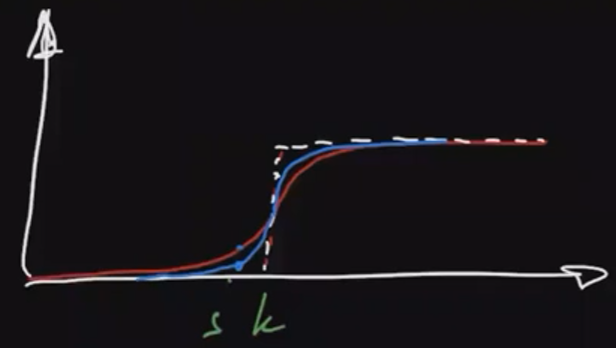
\includegraphics[width=300pt]{picture_10.png}\\
Зависимость дельты от спота за \textcolor{blue}{T=1d}, \textcolor{red}{T=2d} до экспирации
\end{center}  
Delta Bleed - эффект изменения дельты опциона с течением времени, обычно смотрится по дням.\\
Delta Bleed = $\frac{\partial Delta}{\partial T}$\\
\newpage
\section{Vanna}
Пусть у нас есть опцион  USD RUB Call k = 73, s = 72, N = 100m\$, T = 2d\\
Пусть дельта опциона $= D_1$, мы против него держим Short с дельтой $D_1$, чтобы суммарная дельта была 0.
Пусть у нас увеличилась волатильность.\\
\begin{center}  
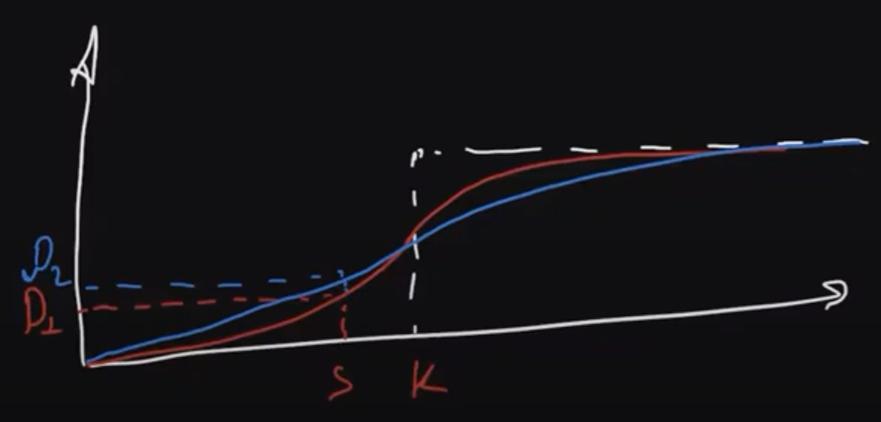
\includegraphics[width=300pt]{picture_11.0.png}\\
График зависимости дельты оп спота
\end{center}
После увеличения волатильности график перешел от красного к синему.\\
Теперь в точке s дельта увеличилась.\\
Тогда теперь дельта портфеля = $D_2 - D_1 > 0$\\
Этот эффект называется Vanna.\\
Vanna = $\frac{\partial Delta}{\partial vol}$\\


Формула не совсем правильная, но помогающая интуитивно понимать дельту: $Delta \sim Prob(exercise)$\\
Она на столько не отличима от правильной, что многие её используют.\\

Пусть у нас есть опцион Call у которого в данный момент спот $s_0$, страйк $k(< s_0)$\\
Давайте поймём, что при увеличении волатильности стоимость этого опциона увеличивается.\\
\begin{center}  
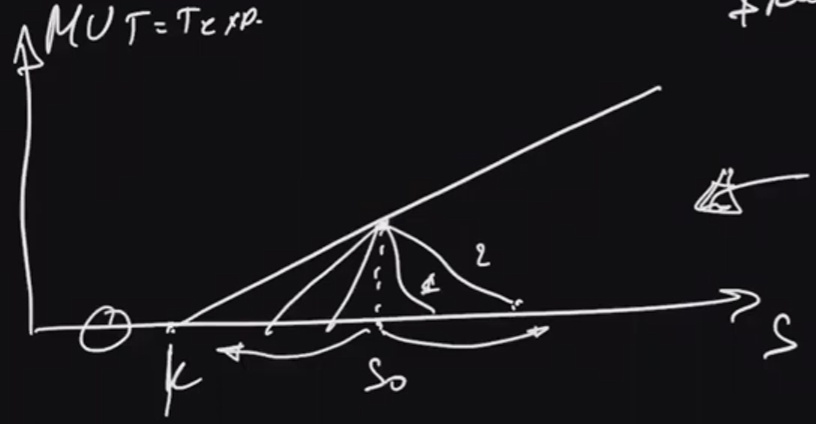
\includegraphics[width=300pt]{picture_11.5.png}\\
\end{center}

Если мы рассмотрим 2 бинарных дерева, ветви которых не вылезают за k(1, 2 на картинке), то можно понять, что их MV будут одинаковыми.
А если наше дерево начинает вылезать за k, то можно понять, что цена начинает расти (и чем дальше левая ветка уходит за k, тем больше будет MV).
\newpage
\section{Модель интерполяции}
Задача модели: Пусть нам даны опционы $X_1, ... X_n$ со стоимостями $MV_1, ... MV_n$.\\
Теперь нам дали новый опцион $X'$, не из ${X_1, .. X_n}$, хотим определить $MV'$.\\
Пример: пусть у нас есть стоимости облигаций одного эмитента в 4 момента времени\\(все кроме центрального)\\
\begin{center}  
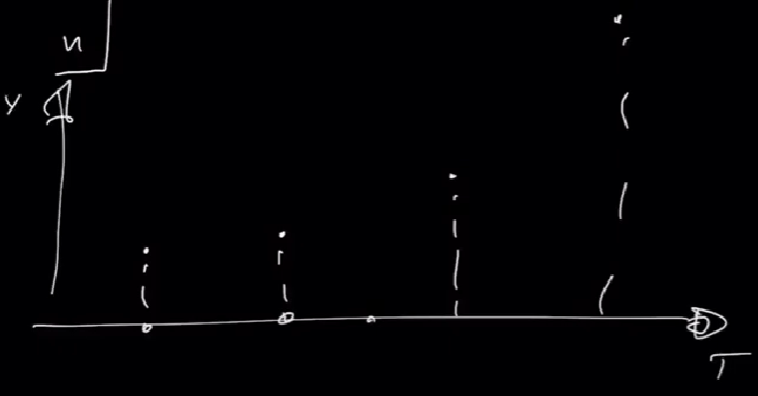
\includegraphics[width=300pt]{picture_12.png}\\
График стоимости облигации от времени.
\end{center} 

\bigskip
Теперь давайте соединим точки одной линией, оценим значение стоимости облигации в центральный момент времени с помощью этой линии.
\begin{center}  
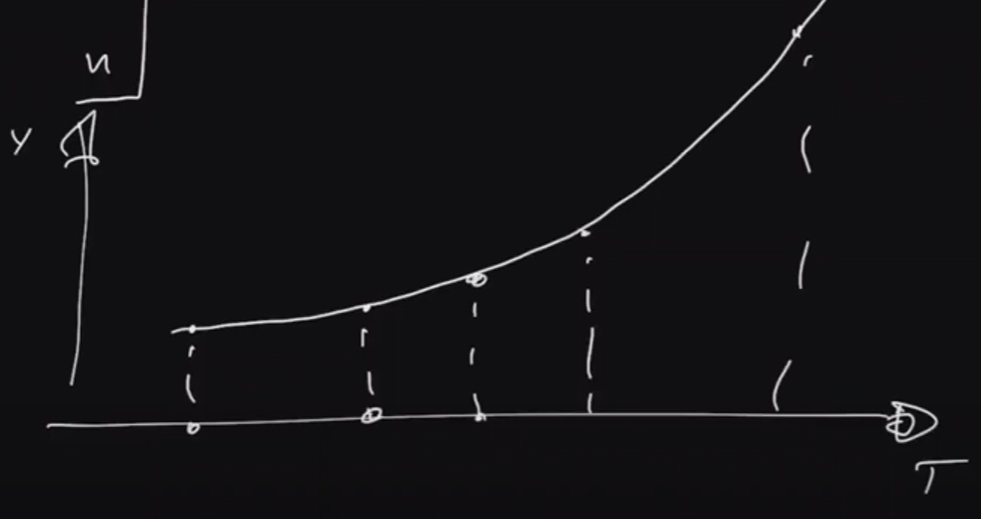
\includegraphics[width=300pt]{picture_13.png}\\
\end{center} 
\end{document}
